\documentclass{standalone}
\usepackage{amsmath,amsfonts,amssymb,mathrsfs,tikz,fancyhdr}
\usepackage{unicode-math}
\usepackage{fontspec}
\usepackage{tikz}
\usepackage{tkz-euclide}
\usepackage{bidi}
\begin{document}
\usetikzlibrary{decorations}%
\noindent%
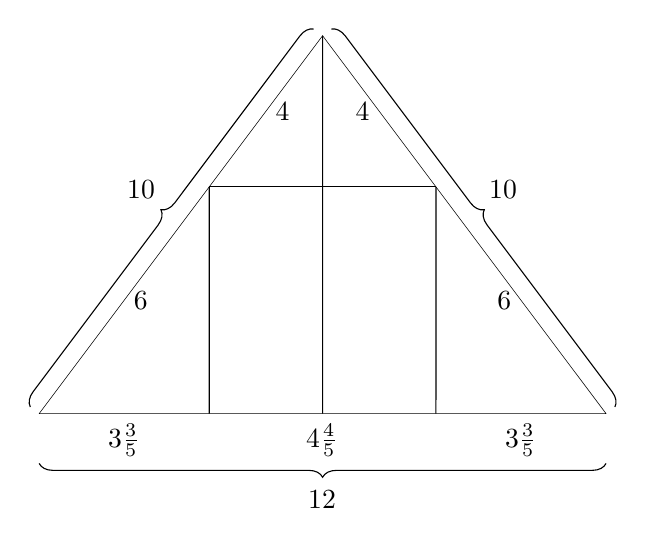
\begin{tikzpicture}[scale=0.6]
 % 1. Define the base points A and B (base side length c)
  \tkzDefPoint(0,0){A}
  \tkzDefPoint(12,0){B}
  % 2. Find vertex C using circle intersections
  % Radius from A equals side b
  % radius from B equals side a
  \tkzInterCC[R](A,10)(B,10)
  \tkzGetPoints{C}{D} % C is the upper intersection
  % 3. Draw the triangle
  \tkzDrawPolygon(A,B,C)
  % the perpendicular
  \tkzDefPointBy[projection = onto A--B](C) \tkzGetPoint{H}
  \draw (C) -- (H);
  % Get point 6 units (60%) along the line
  \coordinate (D) at ($(B)!0.6!(C)$);
  % corresponding perpendicular
  \tkzDefPointBy[projection = onto A--B](D) \tkzGetPoint{DD}
  \draw (D) -- (DD);
  % Get point 6 units (60%) along the line
  \coordinate (E) at ($(A)!0.6!(C)$);
  % corresponding perpendicular
  \tkzDefPointBy[projection = onto A--B](E) \tkzGetPoint{EE}
  \draw (E) -- (EE);
  \draw (E) -- (D);
  % side labels
  % \path (B)--(C) node[midway,above right] {10};
  \draw[decorate,
  decoration={brace,mirror,raise=4pt,amplitude=5pt}]
  (B) -- node[above right=8pt] {$10$}  (C);
  \path (B)--(D) node[midway,left] {6};
  \path (D)--(C) node[midway,left] {4};
  \draw[decorate,
  decoration={brace,raise=4pt,amplitude=5pt}]
  (A) -- node[above left=8pt] {$10$}  (C);
  \path (A)--(E) node[midway,right]  {6};
  \path (E)--(C) node[midway,right]  {4};
  % bottom labels
  \path (A)--(EE) node[midway,below] {$3\tfrac{3}{5}$};
  \node [below] at (H) {$4\tfrac{4}{5}$};
  \path (DD)--(B) node[midway,below] {$3\tfrac{3}{5}$};
  \draw[decorate,
  decoration={brace,mirror,raise=18pt,amplitude=5pt}]
  (A) -- node[below=24pt] {$12$}  (B);
\end{tikzpicture}
\end{document}